\section{Specification}
\label{sec:bus:specification}
Generally our goal is to implement an easy to use bus protocol for fault tolerant application which can 
detect bit errors on a low level and possibly provide forward error correction.
The physical layer of our protocol is a one wire bus accessed via USART, which provides an dominant 
high and an recessive low level.
In the following we differentiate between: 
\begin{enumerate}
 \item Basic access
 \item Fault tolerance: Starvation handling
 \item Fault tolerance: Babbling idiot handling
\end{enumerate}

\subsection{Basic access}
\label{sec:bus:basicaccess}
The access to the bus is provided by arbitration through the Frame ID consisting of Start of Frame (SOF), 
Message Type (or Message ID), the Receivers Node ID and the Sender Node ID, whereat the Node IDs have to 
be globally unique among all Nodes sharing the bus.
Then the payload length in byte, the actual payload and a 32-bit-CRC checksum are transmitted (see section \ref{sec:bus:messageformat}).\\

\begin{figure}[h]
\centering
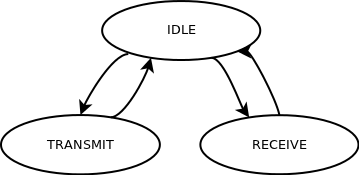
\includegraphics[width=0.6\textwidth]{../images/abstract_statemachine.png}
\caption{Abstract protocol state machine.}
\label{fig:bus:basicaccess:abstractstatemachine}
\end{figure}

Depicting an abstract state machine (given in figure \ref{fig:bus:basicaccess:abstractstatemachine}) we outline three cases:
\begin{enumerate}
 \item Only one node wants to transmit data and the bus is free: Node \textit{A} knows that the bus is free by 
observing the bus since startup. \textit{A} starts to write Start of Frame, MessageID, ReceiverNodeID, SenderNodeID  
to the bus and listens bit wise for the data last written.
       If the bit received equals the bit written \textit{A} knows the bus currently is dominated by itself and 
the arbitration can continue. After arbitrating the whole FrameID every Node currently connected to the bus is 
in the RECEIVE\_STATE except \textit{A} which is in the TRANSMIT\_STATE of the state machine.
       \textit{A} can now send the rest of the message without being interrupted by another node.

 \item More than one node wants to transmit data: Both nodes \textit{A} and \textit{B} start to send 
their Frame ID. Since the Node IDs have to be unique one of the two nodes does not read back the bit written on the bus and changes to the RECEIVE\_STATE. The further scenario is like the one described above.

 \item A node wants to transmit data during another node's already transmitting: Since all nodes connected to the bus are in the RECEIVE\_STATE while another node is sending the node has to wait until the other node currently sending has finished.

 \item Node \textit{C} just powered on and has a wrong state within the protocols state machine. Hence it does not know anything about the communication going on at the moment, leading to the fact of not being capable to decide when he is allowed to arbitrate the bus without violating another transmission.
       If \textit{C} wants to send, it has to wait a predefined time for which the bus must be unused. 
If \textit{C} wants to read, it waits for the next \textit{Start of Frame} occurrence. From this time on \textit{C} has the correct state in the protocols state machine.
\end{enumerate}


\subsection{Fault tolerance: Starvation handling}
\label{sec:bus:ftnsh}
Since the whole network starves in case of a fault at the sending node, e.g. due to a hang up or a power off, during transmission as well as on power on of the very first node, we have to ensure proper operation after some time.
For this purpose a routine is called after each receipt and sets a timer or watchdog for the time interval allowed till the next receipt.
In case the message has been transmitted correctly the timer or watchdog can be deactivated.
In case the sender node stucks during message transmission the timer or watchdog triggers an interrupt resetting the state in the protocols state machine which offers the receiver nodes to initiate or wait for a new transmission.
Another advantage is a faster integration of new nodes, since a new node does not have to wait for the \textit{Start of Frame} of another message to synchronize to the bus protocol because it can set its timer or watchdog and initiate a new transmission after the configured timeout.


\subsection {Fault tolerance: Babbling idiot handling}
\label{sec:bus:ftnbi}
\textit{Note: the babbling idiot handling is not part of the protocol implementation}\\

After providing fault tolerance upon the bus protocol like outlined in the sections \ref{sec:bus:basicaccess} and \ref{sec:bus:ftnsh} we want to cover fault tolerance in case of babbling idiots, by providing a simple bus guardian allowing access to the bus only at predefined times.
In case we use a window of 20ms, the bus guardian of a node blocks the active (send) bus access for 20ms after each message sent by the node. The passive access (receive) to the bus is permitted the whole time. An additional majority voting or some other handling to detect babbling idiots can in our current design only be established with additional hard- and software implementations.


\subsection{Message format in a nutshell}
\label{sec:bus:messageformat}
\begin{figure}[htbp]
  \centering
  \begin{bytefield}{24}
     \bitheader{0,3,4,7-8,13-14,19-20,23}\\
     \bitbox{4}{\footnotesize{SoF}}\bitbox{4}{\footnotesize{Type}} \bitbox{6}{\footnotesize{Dest ID}} \bitbox{6}{\footnotesize{Src ID}} \bitbox{4}{\footnotesize{Len}}\\
     \bitbox[lrt]{8}{\footnotesize{Data<0>}} \bitbox[lrt]{8}{\footnotesize{Data<1>}} \bitbox[lrt]{8}{\footnotesize{...}}\\ 
     \skippedwords \\
     \bitbox[lrb]{8}{\footnotesize{...}}\bitbox[lrb]{8}{\footnotesize{Data<Len-2>}}\bitbox[lrb]{8}{\footnotesize{Data<Len-1>}}\\
     \bitbox[lrb]{8}{\footnotesize{CRC<0>}}\bitbox{8}{\footnotesize{...}}\bitbox{8}{\footnotesize{CRC<3>}}\\
   \end{bytefield}
  \caption{Layer2 message format}
  \label{figure:bus:messageformat}
\end{figure}

As shown in figure \ref{figure:bus:messageformat} the message consists of

\begin{enumerate}
 \item Start of Frame
 \item Message Type 
 \item Receiver Node ID
 \item Sender Node ID
 \item Data Length
 \item Data[0..N]
 \item CRC
\end{enumerate}

The \textit{Start of Frame}, \textit{MessageType}, \textit{ReceiverNodeID} and \textit{SenderNodeID} are part of the so called FrameID uniquely identifying all messages transferred on the bus.
The Field DataLength holds the length of the Payload following in bytes. The message is concluded by the 4-Byte long CRC-checksum.

\subsection{Requirements}
\label{sec:bus:requirements}

